\documentclass[a4paper,12pt,hidelinks]{report}
\usepackage{graphicx}
\usepackage[parfill]{parskip}
\usepackage[backend=bibtex,style=ieee]{biblatex}
\usepackage{fancyhdr}
\usepackage[top=3cm,bottom=3cm,left=3cm,right=3cm,headheight=15pt]{geometry}
\usepackage{gentium}
\usepackage{titlesec}
\usepackage{placeins}
\usepackage{caption}
\usepackage{subcaption}
\usepackage{textcomp}
\usepackage[UKenglish]{isodate}
\usepackage{blindtext}
\usepackage{pdflscape}
\usepackage{tabularx}
\usepackage{longtable}
\usepackage{pdfpages}

\usepackage[pdftex,pdfauthor={Dale Mark Peters (Student Number 120062861)},pdftitle={SE31520 Assignment Documentation | Aberystwyth University},pdfcreator={pdflatex}]{hyperref}

\title{SE31520 Assignment Report}
\author{Dale Mark Peters}
\graphicspath{{/home/dale/university/se31520/assignment/report/images/}}

\bibliography{bibliography}
\captionsetup{width=0.8\textwidth,font={small}}

\titleformat
{\chapter}
[block]
{\bfseries\huge}
{\thechapter}
{3ex}
{}
[]

\pagestyle{fancy}
\fancyhf{}
\lhead[LO]{\leftmark}
\rhead[RE]{\rightmark}
\cfoot{\thepage}
\begin{document}

\maketitle

\tableofcontents\newpage
\chapter{Introduction}
    This document it written to accompany the software I have written for the SE31520 (Developing Internet Based Applications) 2015-2016 assignment. In this
    document, I will describe the architecture and justify the design of my web application and RESTful APIs developed, and will then go on
    to explain the testing strategy used for my applications and give the results of the tests. Finally, I will give an evaluation of how well the requirements
    were met and how well I have done in the assignment.

    In this assignment, I was tasked with the design and implementation of a web application (My Alcohol Free Wines - from now on called MAF) that allows users to find the cheapest prices
    for the non-alcoholic wines they wish to buy. This had to be done by comparing the prices of one identical wine from two different suppliers and displaying the
    cheapest one in the MAF wines listing page. From the wines listings page, the idea was that they can then place their desired wines into their basket and place
    an order, where an `order' consists of sending the details of the purchase and the customer details to the relevant supplier via a RESTful request.

\chapter{Design/Architecture}
    \section{Data Models (Classes)}
    From the specification of the assignment and the system that needs to be implemented, some of the models that needed to be considered were clear.
    These are detailed in this section.
    
    \subsection{Wine}
    The most important of the models to be implemented in the application was the Wine model, which represents a product MAF sells. Most of its attributes were
    can be represented by a string as they are textual attributes of the product. Both descriptions, the bottle size, the origin country, the bottle size, the supplier
    and the grape types can all be represented textually, so I chose a string representation for these.
    
    The price field, however, could be a decimalised amount, so I chose a float representation for these. Also to be stored was the suitability for vegetarians, which 
    is a binary concept, so I chose a boolean representation for this. 
    
    A field I added but is not mentioned in the specification is the some sort of unique identifier to distinguish the same product from
    two difference suppliers. I therefore added a barcode field so that a wine from a particular supplier could be compared to the same wine from the other
    supplier which might have different information. I chose a string representation for this to cover cases where it might begin with a 0.

    \subsection{Customer}
    I have implemented a customer model to represent the customers who might be purchasing from MAF. All the information to be stored about customers was
    to be stored in the form of a string, as all the information to be stored about customers is textual. Another field I had to add to the database for this
    model but wasn't specified in the specification was the password digest field, which is required by the Ruby bcrypt gem to hash the customer passwords.
    It also makes sense that each customer holds a basket, so I added this field to the database to hold the foreign key reference to the user's basket id.

    \subsection{BasketItem}
    It is clear from the specification that the basket in the MAF application could potentially hold several Wine items if the customer wants to add
    several wines to their basket. It is therefore necessary to have a model that links these two tables up. By having this in a separate table, I
    can have as many items as desired in the table without having to have a separate column for each product in the basket. In the way I have designed it,
    the database table just needs two foreign key references - one specifying which wine the item of the basket represents, and the other representing the
    basket it belongs to.

    \subsection{Basket}
    There isn't really much information about what information should be stored about a particular basket in the specification, other than that
    it belongs to a user and that it contains many items. It can therefore be seen as just a container for BasketItem objects in the application,
    so each basket can potentially have multiple BasketItems. It is for this reason that I have declared in the Basket model that it has many
    BasketItems.

    \section{Controllers}
    With Ruby on Rails being a Model View Controller framework, it was important to define several controllers for use in the application.

    \section{Use Case Diagram}
    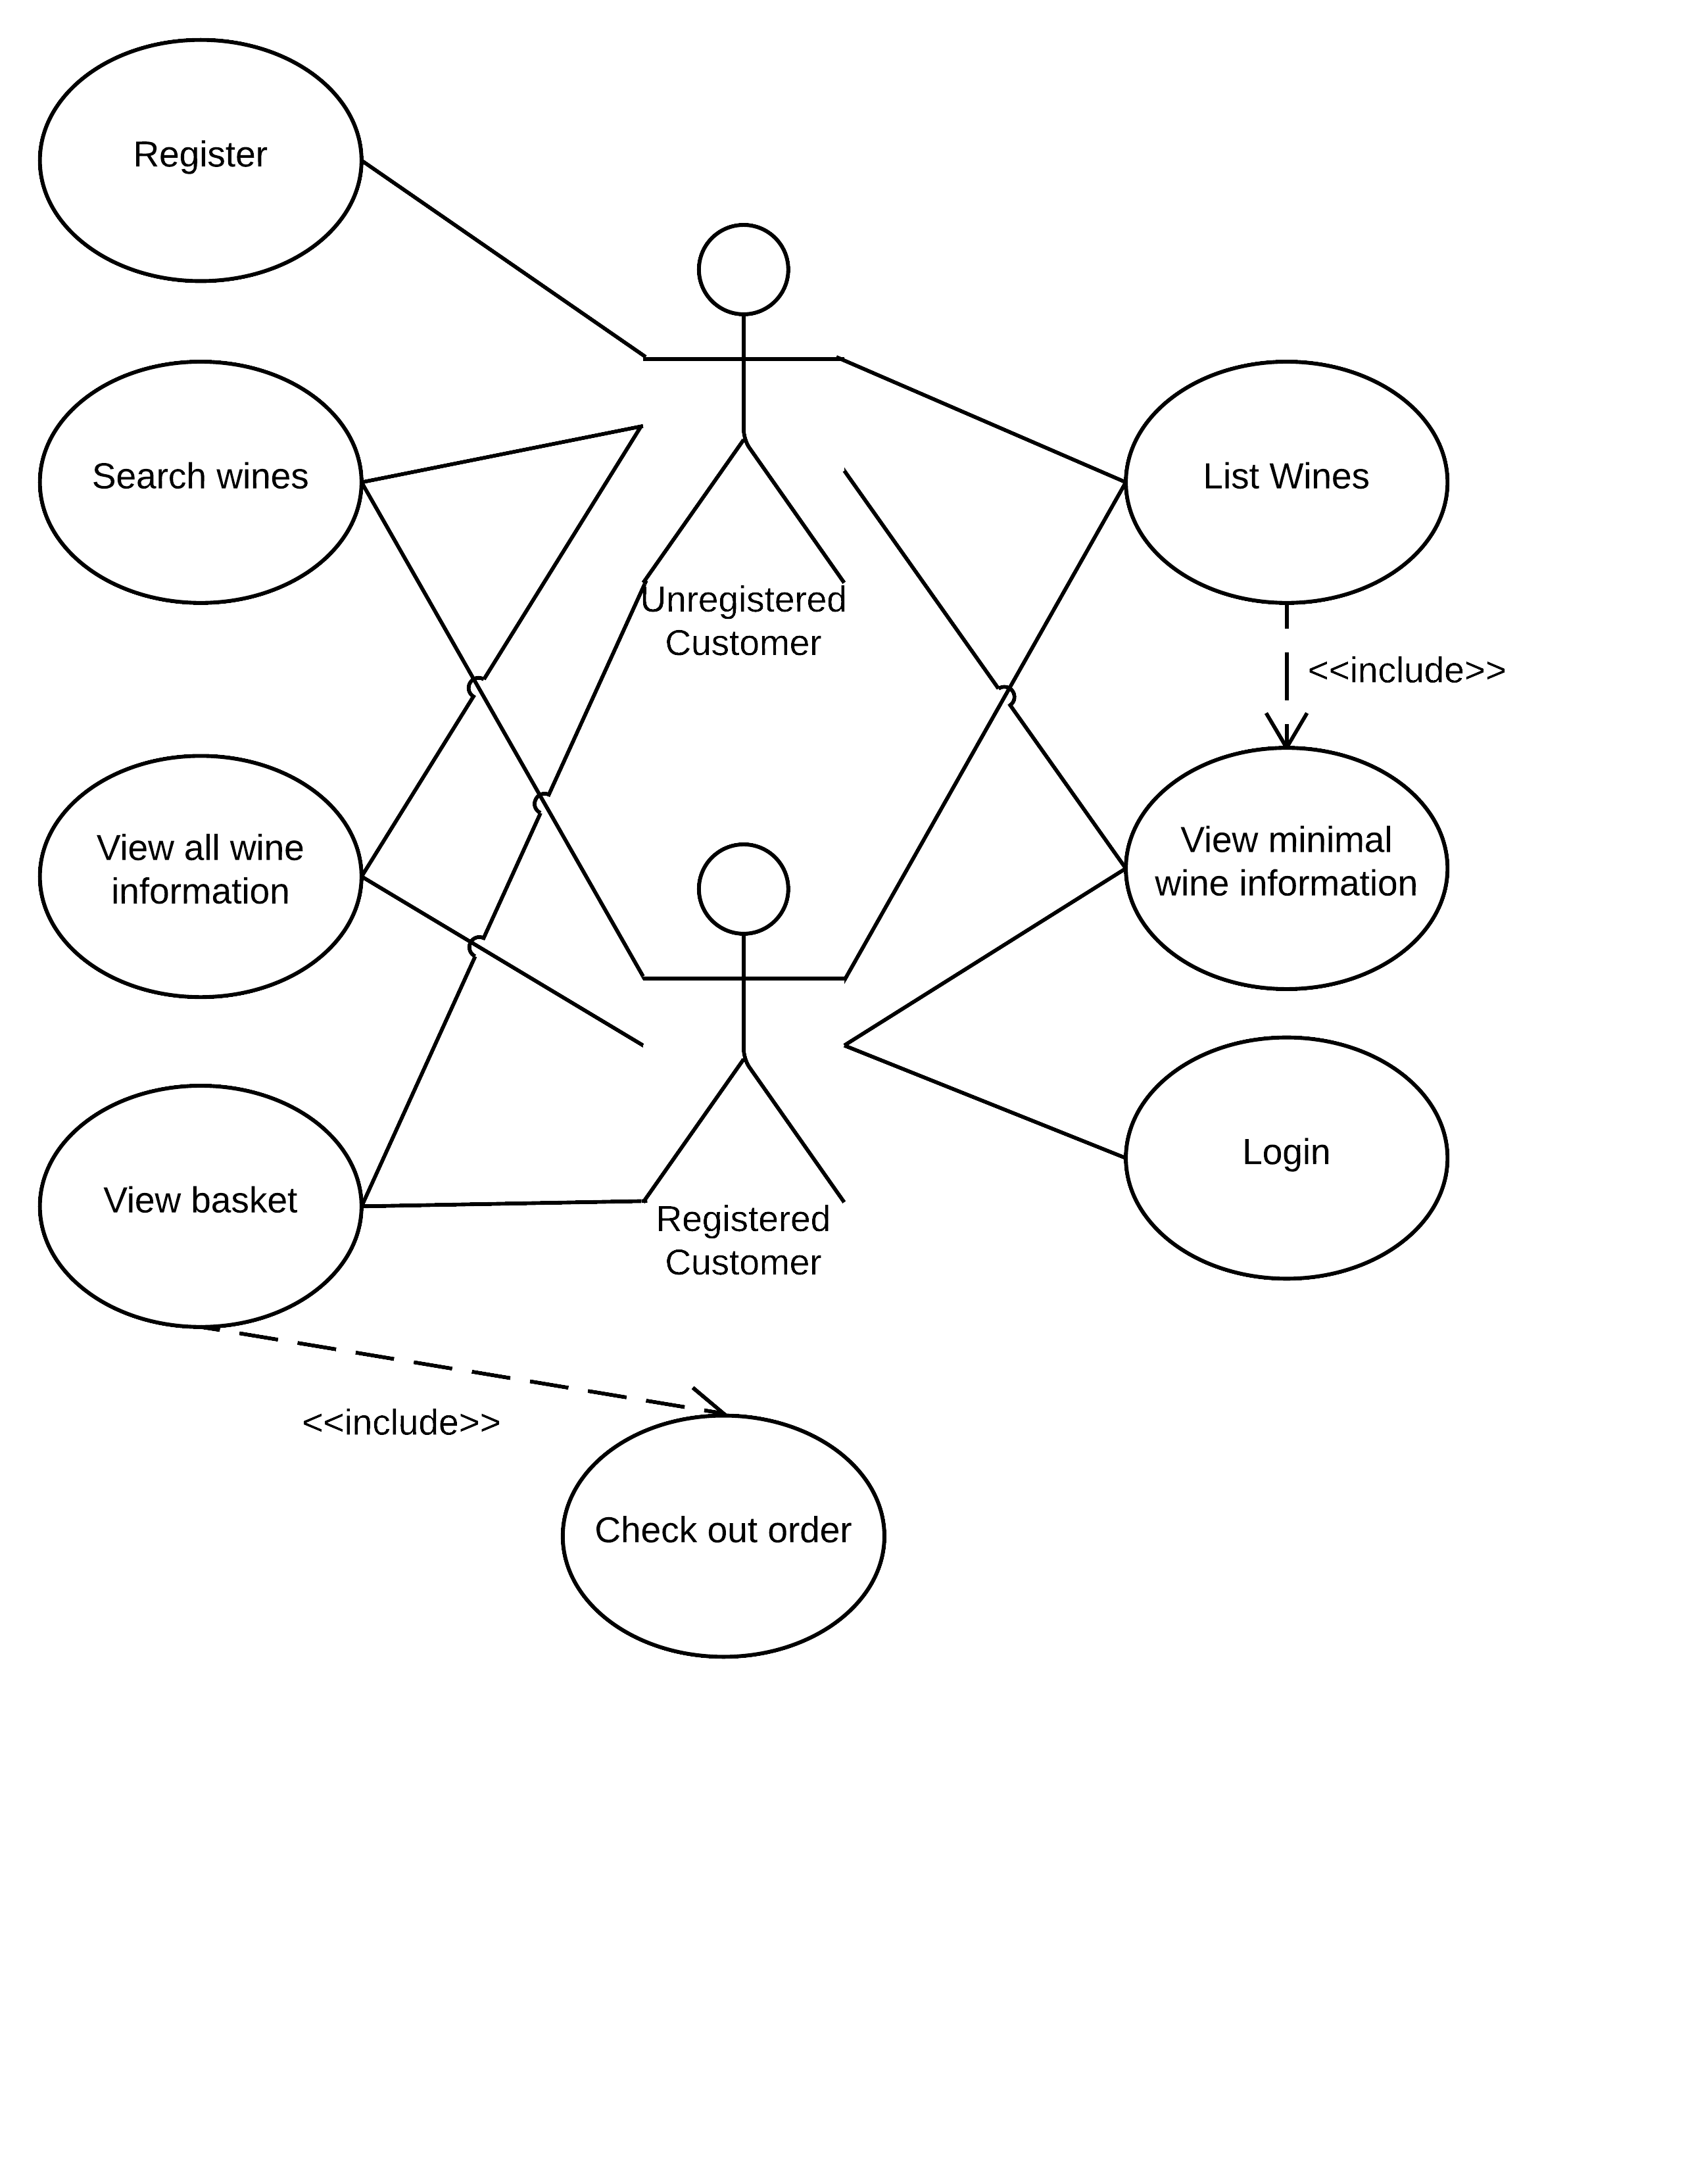
\includegraphics[scale=0.60]{use-case-diagram.png}

    \section{Architecture Diagram}
    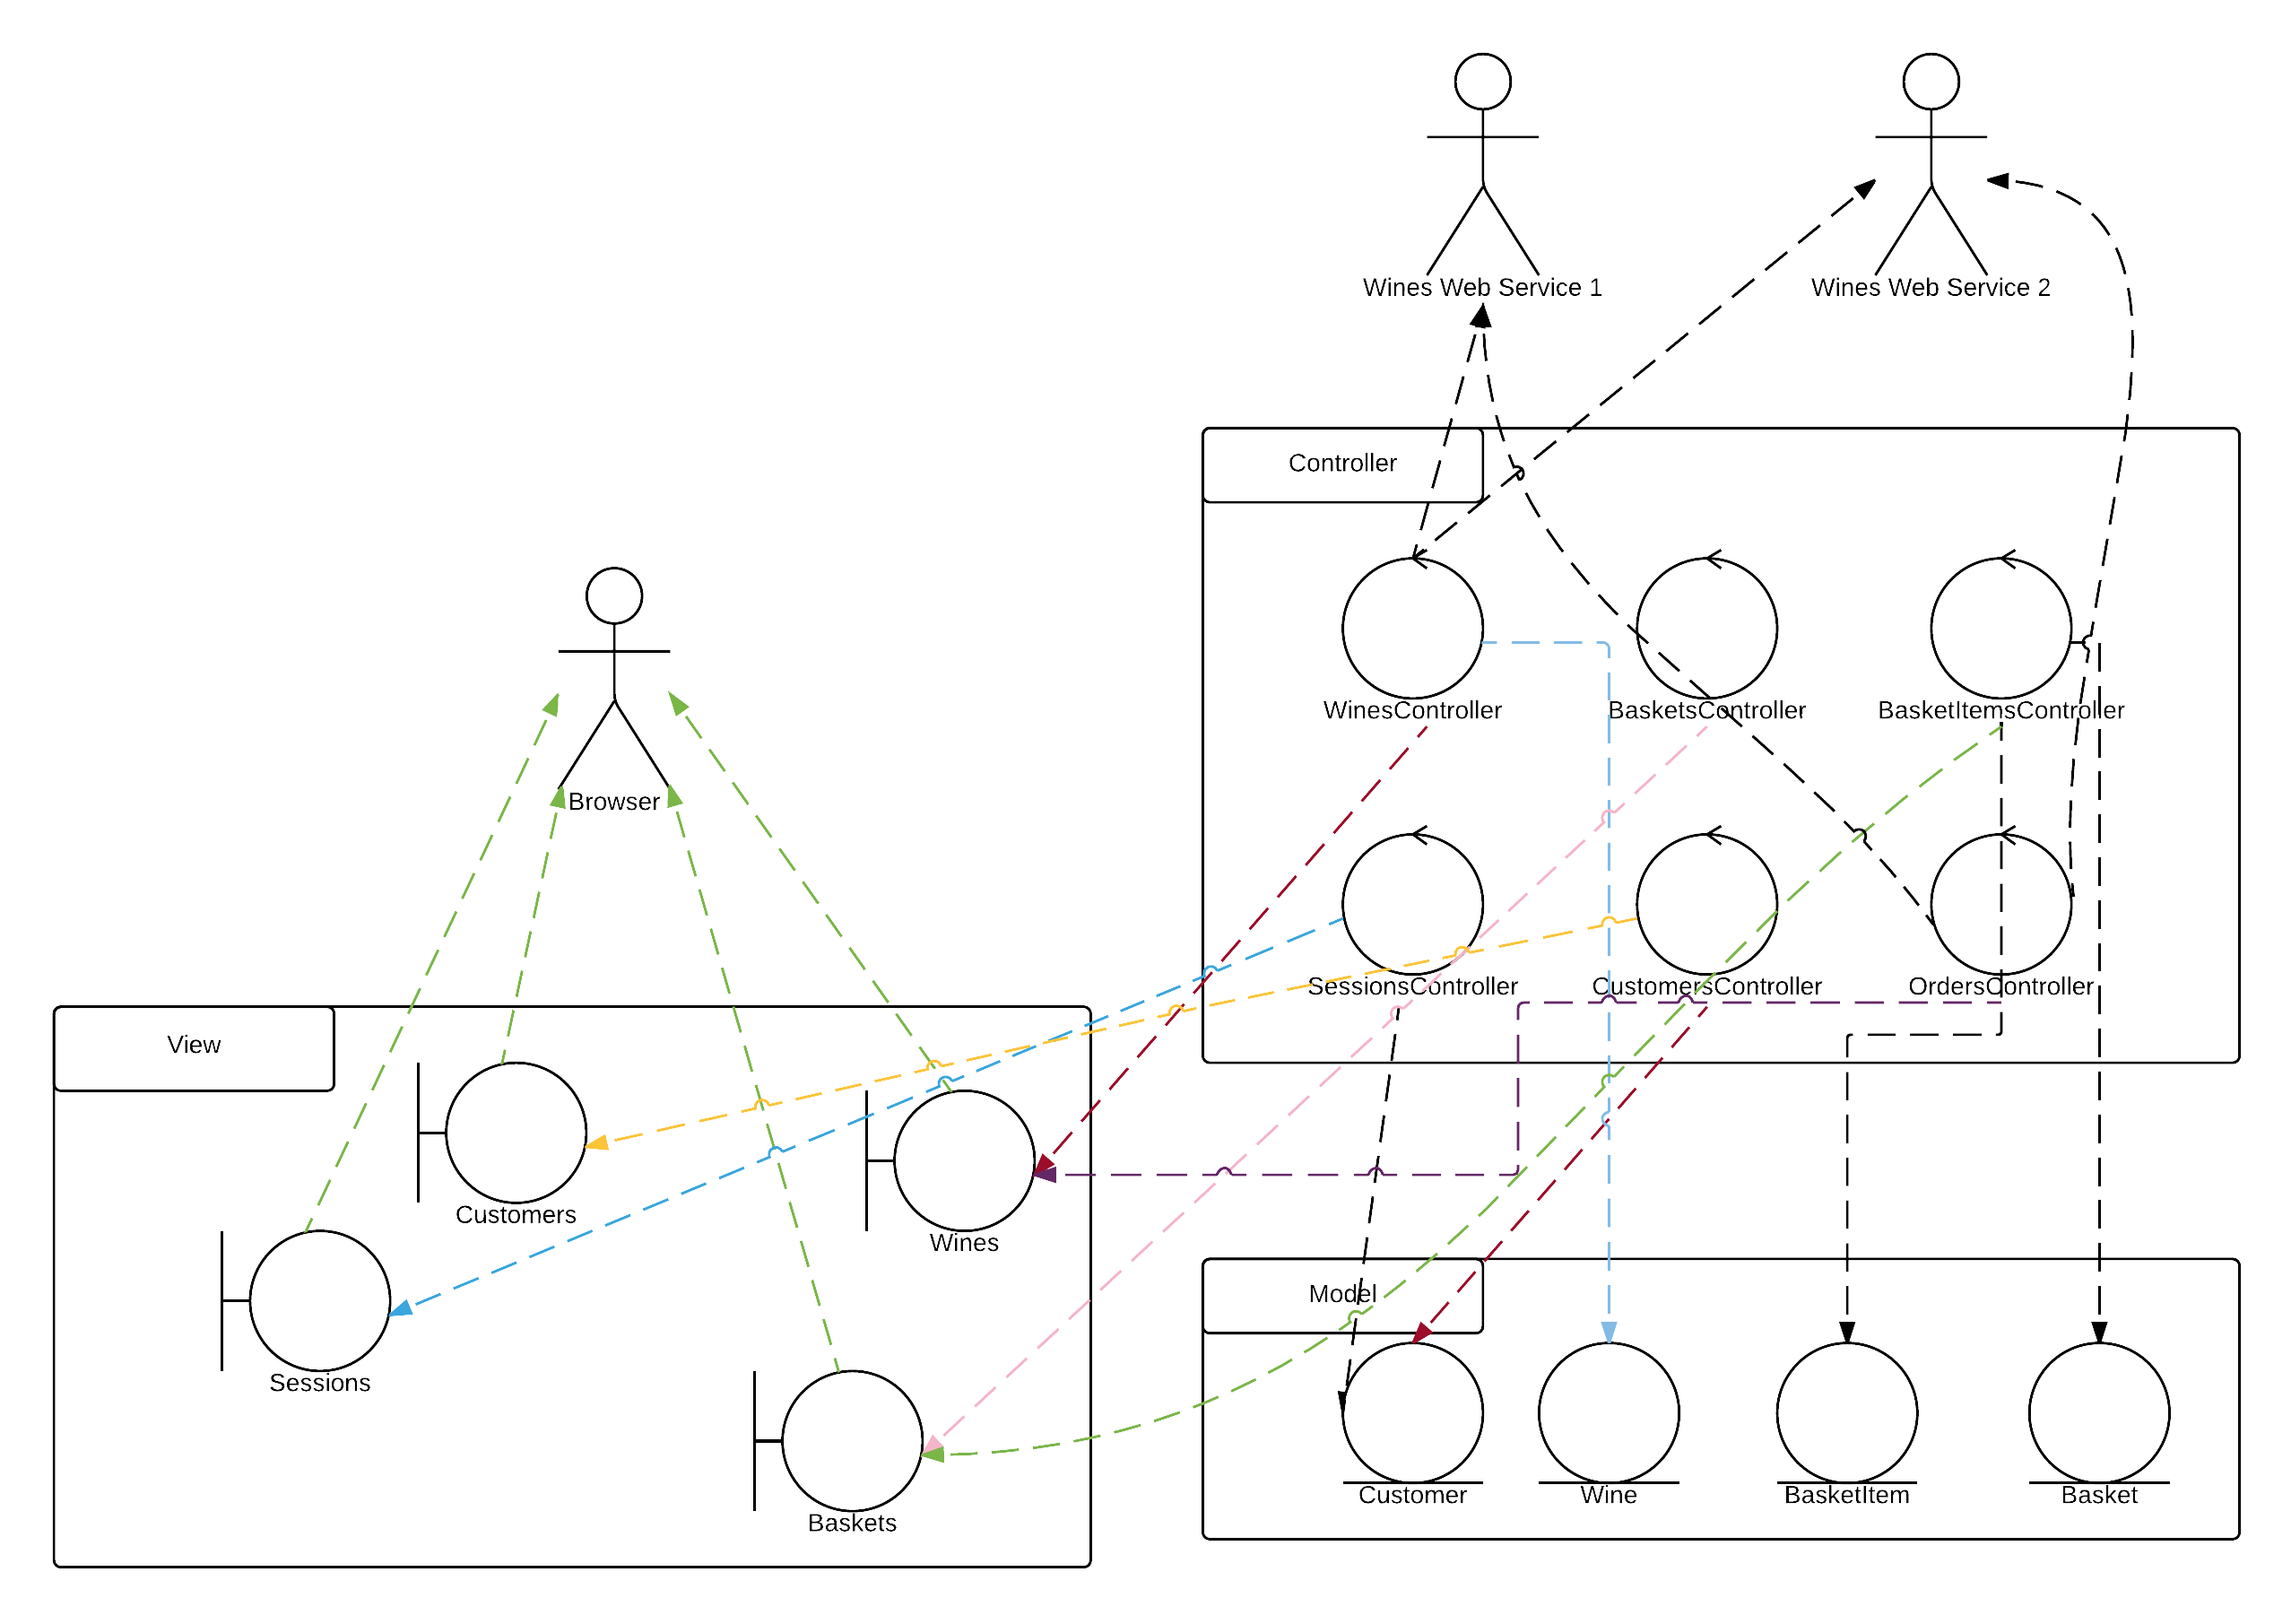
\includegraphics[width=\textwidth]{architecture-diagram.png}

    \section{My Alcohol Free Wines}
    \subsection{Routes}
    This section details the routes that are used in the application.

    \section{RESTful Supplier Web Services}
    As previously mentioned, another part of this assignment was to develop two external RESTful HTTP web services (the suppliers to MAF) which
    supply MAF with all the information on the wines they sell. They also needed to have the capability of receiving order details from MAF when the
    user clicks the checkout button in their cart.

    My two APIs use exactly the same implementation (identical code), and have a HTTP GET route (\url{http://localhost:5000/wines/} and \url{http://localhost:5001/wines/} 
    defined for the supply of wine information to MAF, and a HTTP POST route (\url{http://localhost:5000/orders/} and \url{http://localhost:5001/orders/}).
    Both of these supply and receive data in the form of JSON objects. The reason for this choice was because for each JSON object, there is significantly less
    text than XML and it is good enough for representing the simple nature of the data to be sent between the systems.

    The two services were written in Python, using the \textit{Flask} framework \cite{flask-framework}. I chose to implement these in Python because over my industrial 
    year, I gained experience in this language and it is one I feel confident in. It also didn't require me to write very much code for the web services, compared to the likes of
    Java, for example, so development time was minimal. Whilst I'd had experience in writing software in Python before, I'd never developed a RESTful API with Flask,
    so I had to follow a tutorial to help me with this \cite{flask-tutorial}. The orders sent to the server are not stored when received in this prototype, as this
    is not a requirement of the assignment. Rather, the orders are stored in memory when received. The wines are also stored in memory when the web service server is
    started. \textbf{STORE IN JSON FILE AND CHANGE THIS IF HAVE TIME}. If I had the time, I would have stored these in a separate JSON file and read this in when the service
    starts, so as to reduce the amount of text in the service code. The data in the two applications is different so that the two suppliers' prices can be compared.

\chapter{Third Party Libraries/Code/Assets}
    Whilst doing this assignment, in order to reduce the amount of time it took me to develop the application, I used several third party
    Ruby on Rails gems in addition to the ones that are in a default Rails project. These are listed in the Gemfile, but are also as follows:
    \begin{itemize}
        \item \textbf{rest-client}: Used for the sending of requests from the MAF application to the two RESTful APIs.
        \item \textbf{bcrypt}: Used for the encryption of the customer's user name and password.
        \item \textbf{will\_paginate-bootstrap}: Used for the Bootstrap-style pagination of the wines in the wines listing page.
        \item \textbf{activerecord-session\_store}: Used to store sessions in a database.
        \item \textbf{will\_paginate}: Used for pagination of the wines in the wines listings page
    \end{itemize}

    For the styling of the website, I used Bootstrap CSS, which is contained in the files with names beginning with `bootstrap' in the app/assets/stylsheets
    directory. This was obtained from \cite{bootstrap}.

    The image for the wine was obtained from \cite{wine-image}.

    I also followed tutorials and the book recommended in the reading list of this module in the implementation of this assignment. I have 
    commented in the code to acknowledge where I have based my code on other people's examples. The particular parts of the assignment I
    needed to do this for were the implementation of the basket and the implementation of the login and log out functionalities. For the
    basket functionality, I used one of the recommended books for the module (\cite{agile-web-dev}), and for the logging in a logging out functionality
    I used an online tutorial, located at\cite{online-ruby-book}.



\chapter{Testing}
    \section{Test Strategy}
    \section{System Test Table}
    To create the system test table, I looked at each of the functional requirements given in the specification for the
    assignment and identified the key parts of each requirement that could be tested. Some of the functional requirements can
    be split into several different tests, so I have done this where necessary. For each of the described tests, I followed the contents
    of the `Input' column and recorded the results in the table. This table can be found in the Appendices of this document.

\chapter{Self Evaluation}
    \section{Screencast}
    \section{Design}
    In hindsight, could have had a separate Supplier model, stored in the database so that each has its own unique identifier. Each Wine would
    then have a foreign key reference to a supplier id. This would have made it easier to identify which of the two suppliers to send the 
    order to when the customer checks out their order.

    \section{MAF Implementation}
    \section{Supplier Implementations}
    \section{Testing}
    \section{Flair}

\printbibliography

\titleformat
{\chapter}
[block]
{\bfseries\huge}
{Appendix \thechapter:}
{3ex}
{}
[]
\appendix
\chapter{System Test Table}
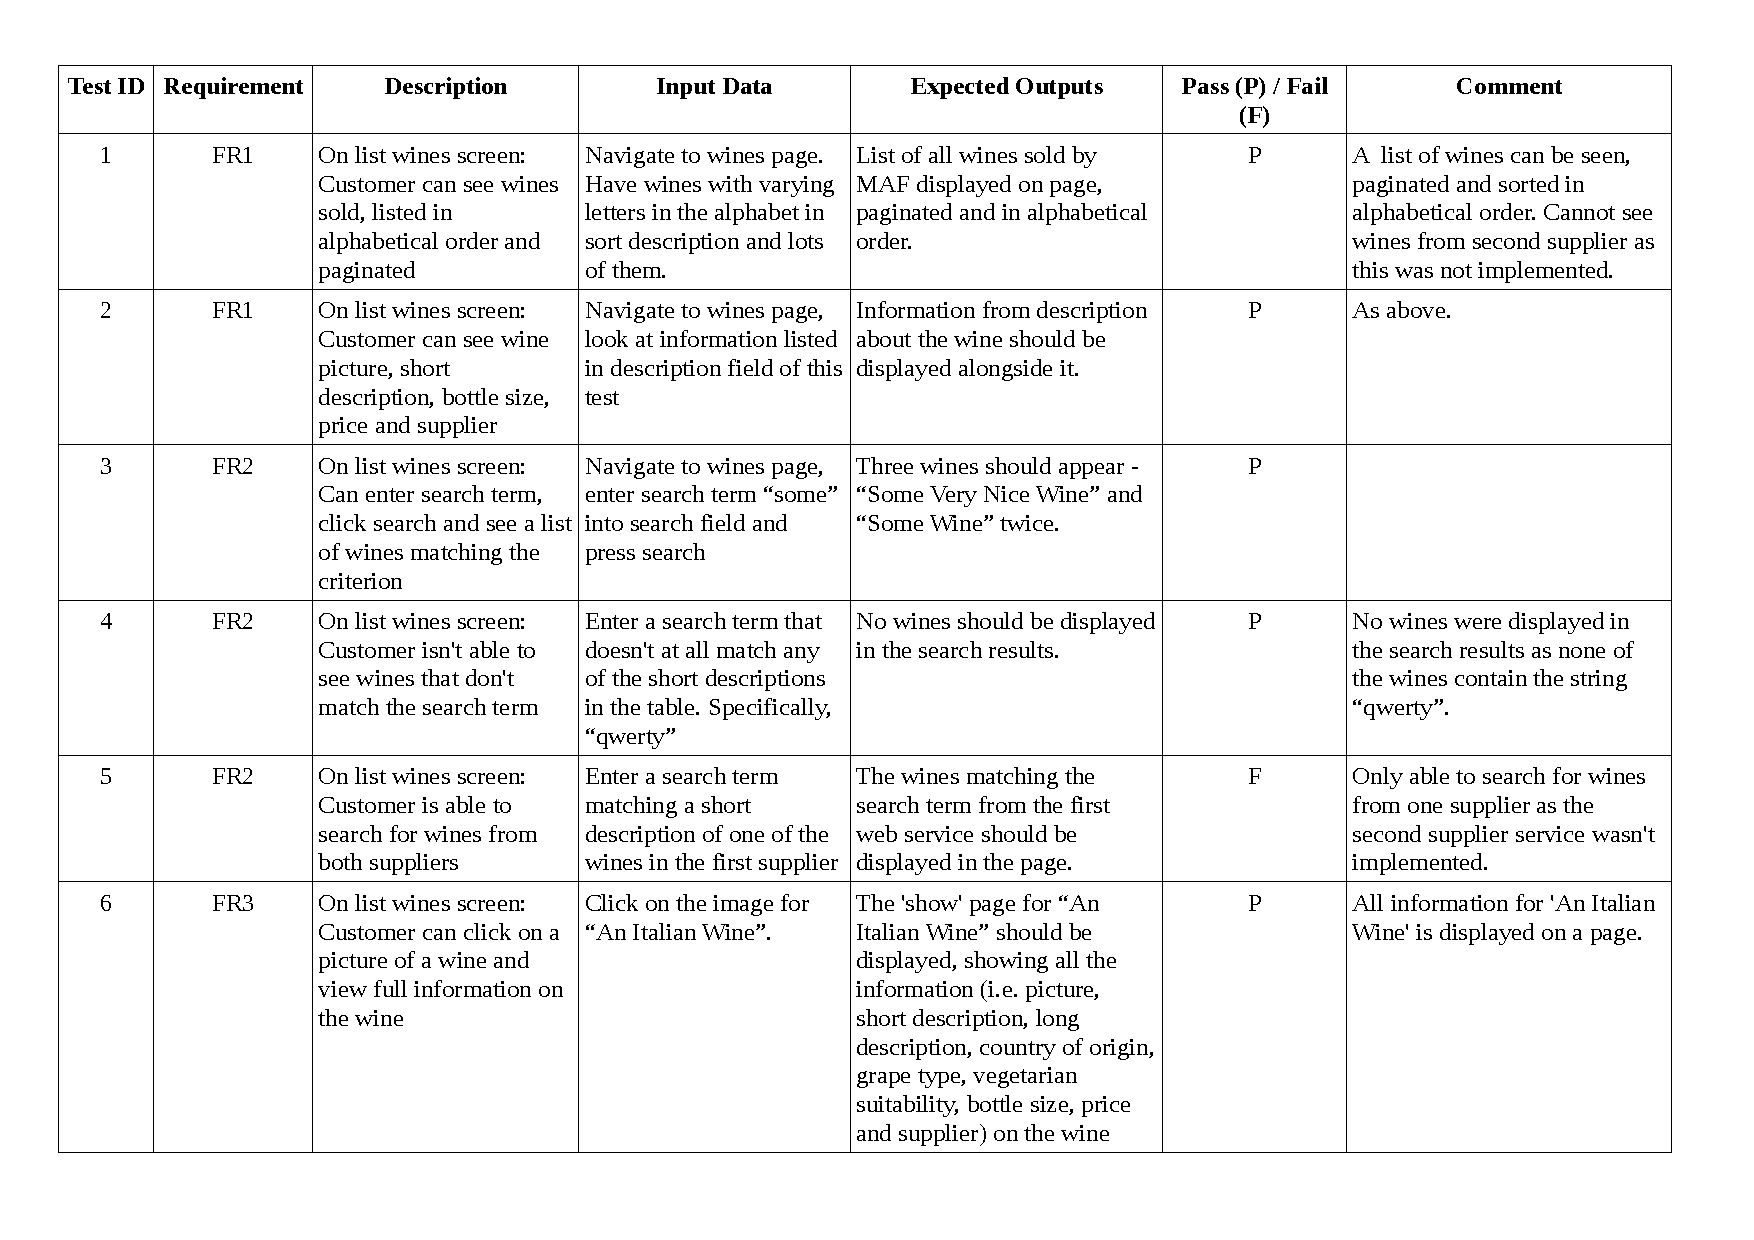
\includepdf[pages={-}, angle=90]{images/test-table.pdf}

\end{document}
